\documentclass[letterpaper,10pt]{article}

\usepackage{enumitem}
\usepackage{titling}
\usepackage{listings}
\usepackage{url}
\usepackage{hyperref}
\usepackage{setspace}
\usepackage{subfig}
\usepackage{sectsty}
\usepackage{pdfpages}
\usepackage{colortbl}
\usepackage{multirow}
\usepackage{multicol}
\usepackage{relsize}
\usepackage{amsmath}
\usepackage{wasysym}
\usepackage{fancyvrb}
\usepackage[yyyymmdd]{datetime}
\usepackage{amsmath,amssymb,amsthm,graphicx,xspace}
\usepackage[titlenotnumbered,noend,noline]{algorithm2e}
\usepackage[compact]{titlesec}
\usepackage{XCharter}
\usepackage[T1]{fontenc}
\usepackage[scaled]{beramono}
\usepackage[normalem]{ulem}
\usepackage{booktabs}
\usepackage{tikz}
\usetikzlibrary{arrows,automata,shapes,trees,matrix,chains,scopes,positioning,calc}
\tikzstyle{block} = [rectangle, draw, fill=blue!20,
text width=2.5em, text centered, rounded corners, minimum height=2em]
\tikzstyle{bw} = [rectangle, draw, fill=blue!20,
text width=4em, text centered, rounded corners, minimum height=2em]

\definecolor{namerow}{cmyk}{.40,.40,.40,.40}
\definecolor{namecol}{cmyk}{.40,.40,.40,.40}
\renewcommand{\dateseparator}{-}

\let\LaTeXtitle\title
\renewcommand{\title}[1]{\LaTeXtitle{\textsf{#1}}}

\lstset{basicstyle=\footnotesize\ttfamily,breaklines=true}

\newcommand{\handout}[5]{
	\noindent
	\begin{center}
		\framebox{
			\vbox{
				\hbox to 5.78in { {\bf ECE 350: Real-Time Operating Systems } \hfill #2 }
				\vspace{4mm}
				\hbox to 5.78in { {\Large \hfill #4  \hfill} }
				\vspace{2mm}
				\hbox to 5.78in { {\em #3 \hfill \today} }
			}
		}
	\end{center}
	\vspace*{4mm}
}

\newcommand{\lecture}[3]{\handout{#1}{#2}{#3}{Lecture#1}}
\newcommand{\tuple}[1]{\ensuremath{\left\langle #1 \right\rangle}\xspace}

\newcommand{\Rplus}{\protect\hspace{-.1em}\protect\raisebox{.35ex}{\smaller{\smaller\textbf{+}}}}
\newcommand{\Cpp}{\mbox{C\Rplus\Rplus}\xspace}


\addtolength{\oddsidemargin}{-1.000in}
\addtolength{\evensidemargin}{-0.500in}
\addtolength{\textwidth}{2.0in}
\addtolength{\topmargin}{-1.000in}
\addtolength{\textheight}{1.75in}
\addtolength{\parskip}{\baselineskip}
\setlength{\parindent}{0in}
\renewcommand{\baselinestretch}{1.5}
\newcommand{\term}{Spring 2023}
\newcommand{\termnumeric}{1235}

\singlespace


\begin{document}

\lecture{ 20 --- Input/Output Buffering and Scheduling }{\term}{Jeff Zarnett}

\section*{Buffering}

Regardless of whether a device is block- or character-oriented, the operating system can improve its performance through the use of buffering. As you may have experienced with Java, the use of a buffer speeds things up quite a lot. A buffer is nothing more than an area of memory that stores data being transferred, whether it is from memory to a device, device to memory, or device to device. 

A buffer is a good way to deal with a speed mismatch between devices. Users type very slowly, from the perspective of the computer, and it would be awfully inefficient to ask the disk, a block oriented device, to update itself on every single character. It is much better if we wait until we have some certain amount of data (e.g., a whole line or whole block or full buffer, whichever it is) and then write this out to disk all at once. 

The write is, however, not instantaneous and in the meantime, the user can still keep typing. Thus, to solve this, the typical solution is \textit{double buffering}, that is, two buffers. While buffer one is being emptied, buffer two receives any incoming keystrokes. Double buffering decouples the producer and consumer of data, helping to overcome speed differences between the two~\cite{osc}.




\subsection*{I/O Scheduling}

As a final note, we sometimes want to schedule I/O requests in some order other than First-Come, First-Served. A simple analogy: Imagine you need to go to the grocery store, the dry cleaners, and the bank. The bank is located 1~km to the west of your current location, and the grocery store is 3~km west. The dry cleaners is in the same plaza as the grocery store. It is obvious that it would be fine to go to the bank, then the dry cleaners, then the grocery store, but not to go to the dry cleaners, then the bank, then the grocery store. The unnecessary back-and-forth wastes time and energy (whether walking or fuel depends on your mode of transportation).

Clearly, the operating system will want to do something similar with I/O requests. It will maintain a structure of requests and can then re-arrange them to be accomplished most efficiently. The literature sometimes refers to this as a queue but... is it really a queue when it does not exhibit the first-in, first-out behaviour\footnote{But I'm kind of strict about my use of grammar and language. Things like ``10 items or less'' signs bother me, because I know it should be ``10 items or \textbf{fewer}''. For those who are fans of \textit{Game of Thrones}, it will probably not surprise you that I like Stannis Baratheon.}? This will, naturally, have some limits: requests should presumably get scheduled before too much time has elapsed even if it would be ``inconvenient''. It might also take priority into account, dealing with the I/O requests of a high priority process even if they are not particularly nearby to other requests. 

In particular, this is important when examining hard disk drive operation. And that will therefore be the next subject we will consider.

\section*{Transforming I/O Requests to Hardware Operations}

In the previous section we discussed the idea of taking a command like \texttt{read} and said it is the job of the device driver to translate this command into a hardware operation. Reading from the file system on disk, for example, requires a few steps. If I want to open a file like \texttt{example.txt}, the file system (not yet discussed) will associate this file with some information about where on the disk this is (a set of disk blocks representing the file). Then, to read the file, \texttt{read} commands can be issued to get those blocks into memory so I can edit it with \texttt{vi}.

The diagram below shows the life cycle of an I/O request:

\begin{center}
	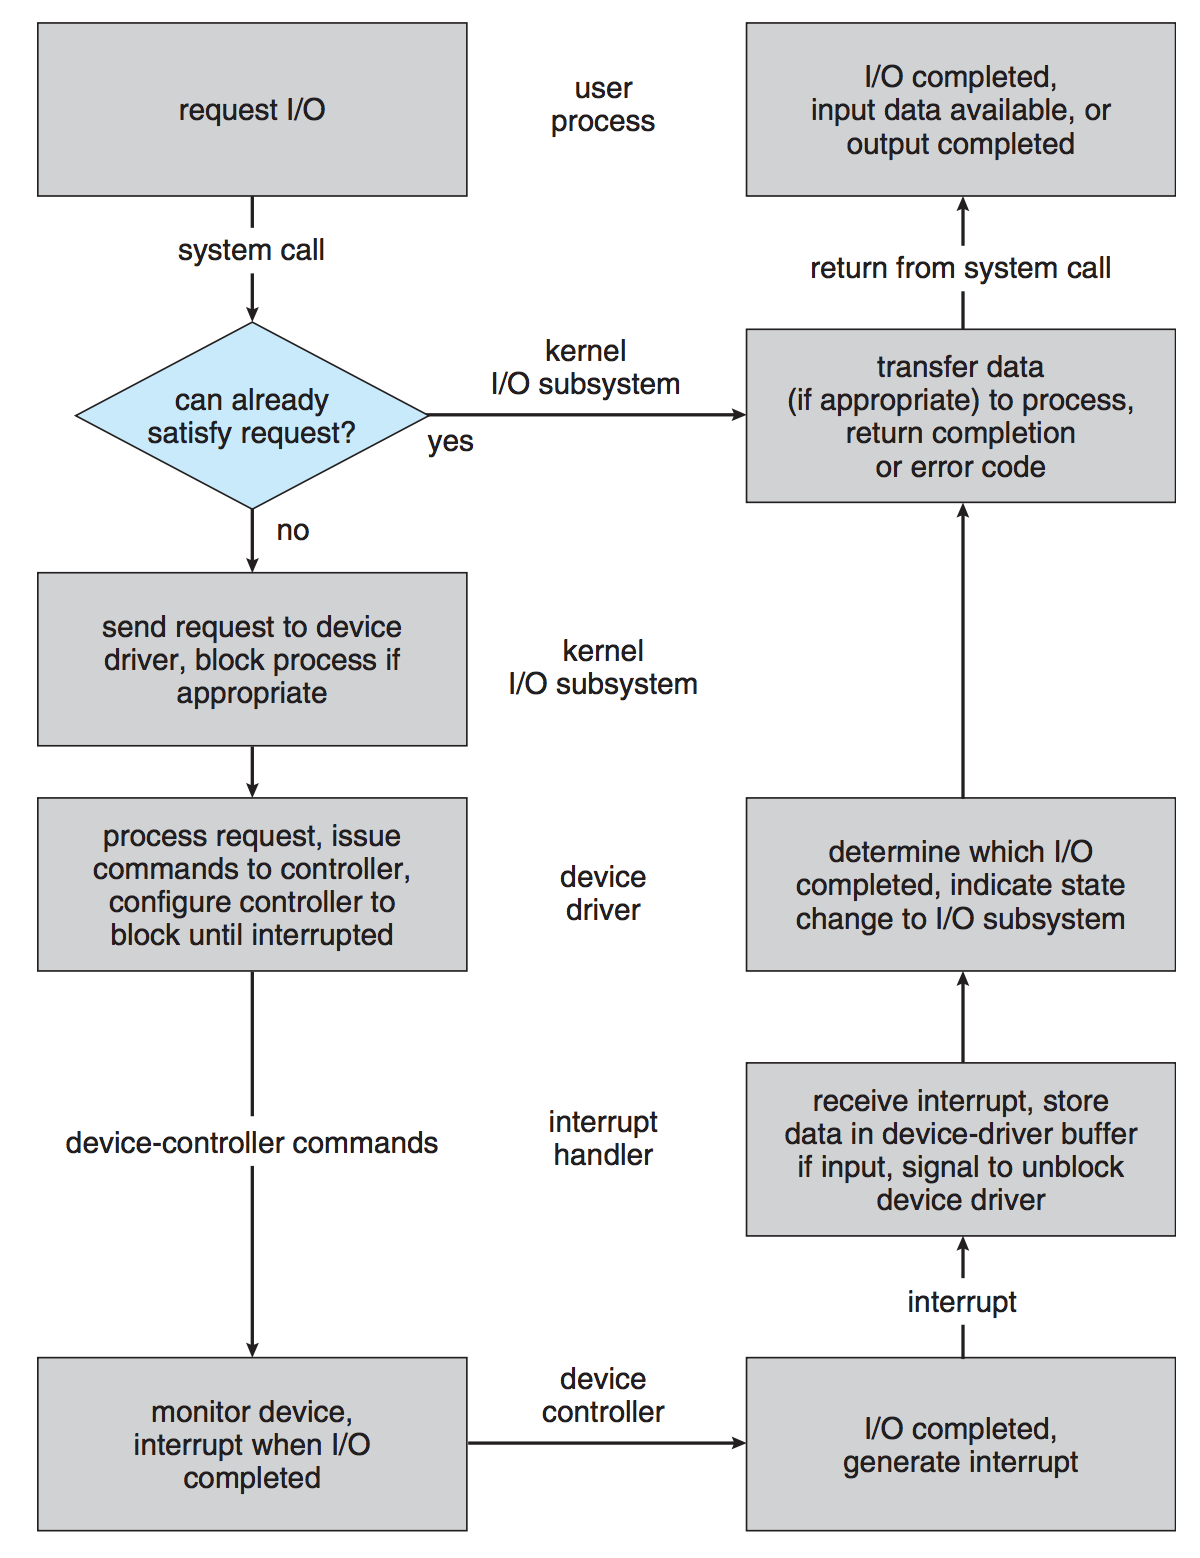
\includegraphics[width=0.65\textwidth]{images/io-lifecycle.png}\\
	The life cycle of an I/O request~\cite{osc}.
\end{center}

In general, the life cycle follows some ten steps from start to finish~\cite{osc}:

\begin{enumerate}
	\item A process issues a \texttt{read} command (assume the file is already open).
	\item The system call routine checks the parameters for correctness. If the data is in a cache or buffer, return it straight away.
	\item Otherwise, the process is blocked waiting for the device and the I/O request is scheduled. When the operation is to take place, the I/O subsystem tells the device driver.
	\item The device driver allocates a buffer to receive the data. The device is signalled to perform the I/O (usually by writing into device-control registers or sending a signal on a bus).
	\item The device controller operates the hardware to do the work.
	\item The driver may poll for status, await the interrupt when finished, or for the DMA controller to signal it is finished.
	\item The interrupt handler receives the interrupt and stores the data; it then signals the device driver to indicate the operation is done.
	\item The device driver identifies what operation has just finished, determines the status, and tells the I/O subsystem it is done.
	\item The kernel transfers the data (or error code or whatever) to the address space of the requesting process, and unblocks that process.
	\item When the scheduler chooses that process, it resumes execution.
\end{enumerate}

\bibliographystyle{alphaurl}
\bibliography{350}


\end{document}